\textcolor{blue}{Problem 2}
\begin{enumerate}
    \item From Figure 4.12, $\mathbb{E}[E_{out}(g^-_{m^*})]$ is initially decreasing. How can this be, if $\mathbb{E}[E_{out}(g^-_{m^*})]$ is increasing in $K$ for each $m$? (10pt)
    \item From Figure 4.12 we see that $\mathbb{E}[E_{out}(g_{m^*})]$ is initially decreasing, and then it starts to increase. What are the possible reasons for this? (10pt)
    \item When $K=1$, $\mathbb{E}[E_{out}(g^-_{m^*})]<\mathbb{E}[E_{out}(g_{m^*})]$. How can this be, if the learning curves for both models are decreasing? (10pt)
\end{enumerate}
\begin{figure}[htbp]
    \centering
    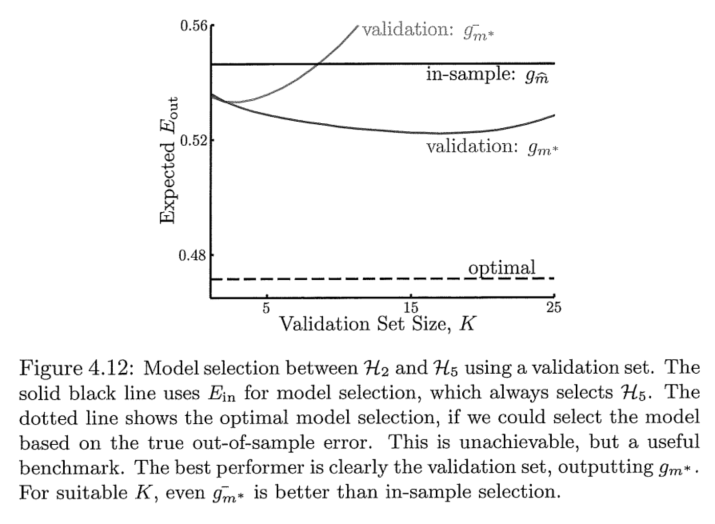
\includegraphics[width=0.8\textwidth]{../fig/figure412.png}
\end{figure}
\par


\textcolor{blue}{Solution}\\
1.\\
(a) Initally, the size of validation set $K$ is quite small, so it would not be able to provide a good estimate of the generalization error. As $K$ increases, the estimate of the generalization error becomes more accurate, so $\mathbb{E}[E_{out}(g^-_{m^*})]$ initially decreases.\\
(b) Similarly to te Problem 1, the size of the total data is fixed, so as $K$ is large enough, then as $K$ increases, there are less points used for training. We can assume that are data points are useful data, so less data points used for training will lead to a worse model. And it is reasonable that the performence of the model both on training set and validation set will decrease. i.e. $\mathbb{E}[E_{out}(g^-_{m^*})]$ increases.

So above all, as $K$ increases, the $\mathbb{E}[E_{out}(g^-_{m^*})]$ is initially decreasing, when $K$ is large enough, $\mathbb{E}[E_{out}(g^-_{m^*})]$ is increasing in $K$ for each $m$ as $K$ increases.

2. The understanding of the notions:\\
The models are $\mathcal{H}_1,\cdots,\mathcal{H}_M$, we first train with training data $\mathcal{D}_{\text{train}}$ to train all models, and use the cross-validation to get the best model $\mathcal{H}_{m^*}$, with error $g^-_{m^*}$ on the validation set $\mathcal{D}_{\text{val}}$. Then the total dataset $\mathcal{D}$ is used for training the model $\mathcal{H}_{m^*}$, and the error on the test set $\mathcal{D}_{\text{test}}$ is $g_{m^*}$.\\
So with the understanding of notions, we can get that:\\
$\mathbb{E}[E_{out}(g_{m^*})]$ is only relevant to the model we selected. When $K$ is small, as $K$ increases, $\mathcal{D}$ is quite close to $\mathcal{D}_{\text{train}}$, so it is similar to $g^-_{m^*}$, so $\mathbb{E}[E_{out}(g_{m^*})]$ decrease as we can choose the good model with cross validation.\\
When $K$ is large enough, as $K$ increases, less useful data are in $\mathcal{D}_{\text{train}}$, although we can choose a good trained model among $\mathcal{H}_1,\cdots,\mathcal{H}_M$, but the best trained model is not good enough, so the error $\mathbb{E}[E_{out}(g_{m^*})]$ on the test set $\mathcal{D}_{\text{test}}$ is increasing.\\

So above all, $\mathbb{E}[E_{out}(g_{m^*})]$ decreases initially, and then it increases as $K$ increases.\\

3. A possible reason is that $K=1$ is too small that even though the models are well trained, the $g_{m^*}$ could have a small $E_{\text{in}}$, but could not make sure that $E_{\text{out}}$ is small.\\
But $g^-_{m^*}$ is trained with cross-validation, so it is more likely to have a good $E_{\text{out}}$ as it is selecting the best model on $\mathcal{D}_{\text{val}}$.
So we have when $K=1$,
$$\mathbb{E}[E_{out}(g^-_{m^*})]<\mathbb{E}[E_{out}(g_{m^*})]$$

\newpage